%!TEX root = ../main.tex

In this chapter we introduce a few technical concepts in order to make our proposed method and what we aim to accomplish more clear.

\section{Augmented Reality}
Augmented Reality is defined as a software system that features a blend of real and virtual objects; the user can interact with it in real time, and it displays a 2D representation of a 3D world for both the real and virtual sides. This is the first definition of AR originally presented by \citep{azuma1997}. \newline
In order to combine real and virtual objects, both worlds must be aligned, in the sense that they must share a common origin for both position and rotation, so that they can coexist in a realistic way within the same image. If the virtual objects present in the real scene are not aligned, the consistency of the whole composition is compromised. \newline
The tracking of real world features as a guideline for alignment in the virtual world is one of the challenges in the field of AR. \citep{zhou2008} have researched the state-of-the-art technologies used for tracking. Different techniques have been used, such as sensor-based tracking, that uses dedicated hardware to feed the software application the position and rotation information it needs. Our method uses vision-based tracking, in which the position and orientation origin of the virtual world are determined by images that are recognized using a computer vision algorithm. These images are named \emph{fiducial markers}. They are divided into the following categories:
\begin{itemize}
  \item \textbf{Binary markers}: Computer-generated black and white images that form patterns. Any combination of at least $8\times8$ black and white pixels that doesn't form a repeating pattern can work as a binary marker.
  \item \textbf{Natural image markers}: A computer vision algorithm extracts features as points, lines, shapes and/or textures in any image that has identifiable elements. This means that the image must have contrasting details spread across the whole image and not form repeating patterns.
  \item \textbf{3D markers}: A small object is analyzed and a point cloud is extracted. During the tracking phase, point clouds are generated from the camera input and matched to the reference cloud. The main advantage is that the viewing angle becomes irrelevant to recognize the marker.
  \item \textbf{Mixed}: Other approaches involving both sensors and vision algorithms have also been used. 
\end{itemize}

While our method does not aim to alleviate the technical challenge of tracking other than existing means, it is necessary to explain the concept for clarity. 

\section{Sensors}
State-of-the-art smartphones and tablets in the market have built-in sensors to perform different kinds of measurements that are helpful for application developers. Such measurements include tracking motion, orientation and other environmental conditions. The sensors that are relevant for our method are the following:\newline
\textbf{Accelerometer}: Measures proper acceleration relative to gravity. Its application in mobile development is to measure motion changes and to detect the orientation of the device relative to the surface of the Earth. It usually consists of 3 orthogonal axes, and therefore can measure acceleration on one, two or three axes. The output is given in m/s\textsuperscript{2}. \newline
\textbf{Gyroscope}: A sensor that is capable of measuring the rate of rotation around a particular axis. It serves the same purpose as the accelerometer, but mobile devices usually have both for more robust measurements. The output is given in rad/s. In our method, both the accelerometer and the gyroscope are used to acquire the $360^{\circ}$  panoramic photograph, making sure that the device is within the same pitch while capturing all the images that will be stitched together to make the panorama. \newline
\textbf{Magnetometer}: It serves the purpose of a compass by measuring the orientation of the device with respect to the Earth magnetic poles. For application development, it is useful to get the heading of the device with respect to the geographic north in a clockwise direction. This heading is an angle expressed in degrees.\newline
\textbf{GPS}: Measures the raw position of the device in three-dimensional Cartesian coordinates where the origin is the center of the Earth. It is used to determine where on Earth the device is located (Country, city, neighborhood, etc.). It needs to have an uninterrupted line of sight, with no electromagnetic interference, to at least 4 out of the 24 satellites in orbit that are used for GPS.

\section{Standard Illuminant}
In order to describe the color of a light source, it is important to have detailed knowledge of the type of illuminant used. The International Comission on Illumination (CIE) defined a number of spectral power distributions, referred to as CIE standard illuminants, to provide reference spectra for colorimetric issues. The illuminants are denoted by a letter or a letter-number combination. Their spectral power distributions (SPD) are normalized to a value of 100 at a wavelength of 560 nm. Illuminants series A through D exist, all of them specializing on a different kind of light source. For our method, the relevant one is series D, as it describes a type of average light source, typically associated to daylight global illumination.\newline
D65 corresponds roughly to the average midday light in western and northern Europe, comprising both direct sunlight and the light diffused by a clear sky in indoors situations. Because of that, it is also called a \emph{daylight illuminant}. The illuminant has a correlated color temperature of approximately 6500 K. Since a standard illuminant is represented as a table of averaged spectrophotometric data, any light source which statistically has the same relative spectral power distribution (SPD) can be considered as a D65 light source. It is important to note that D65 is purely theoretical, there are no actual artificial D65 light sources. The D65 is the white point that we used to convert chromatic information into luminance for the light source detection, as we detail further in section \ref{lsf}.

\section{Panoramic photography}
Panoramic photography is a technique for capturing images with horizontal, and sometimes also vertical, elongated fields of view. While there is no formal definition of the minimum field of view required for a photograph to be considered panoramic, we focus on complete horizontal $360^{\circ}$ captures.\newline
There are different types of panoramic images. The one called wide-format photograph consists of a series of photos taken from the same height, that are then stitched together to appear as a single wide image. The image can subsequently be projected on to a cylinder. This kind of panoramic photograph captures $360^{\circ}$ of the horizontal field of view, while the vertical field of view is dependant entirely on the lens used to capture the individual photographs. Figure 3.1 shows an example of a cylindrical panoramic image. 

\begin{figure}[H]
  \centering
  \setlength{\unitlength}{\textwidth} 
    \begin{picture}(1,0.5)
       \put(-0.1,0){\includegraphics[width=1.3\unitlength]{Figures/pano6.jpg}}
       
    \end{picture}
    \caption{A cylindrical panorama of Trafalgar Square.}
\end{figure}

The type of panoramic image used in our method is called \emph{equirectangular} panoramic image, or spherical panoramic image, due to the fact that the resulting image can be projected on to a sphere. The projection maps meridians to vertical straight lines of constant spacing, and circles of latitude to horizontal straight lines of constant spacing. This kind of projection introduces the types of distortion often seen in spherical projections, such as Mercator, where the poles of the sphere appear bigger than they really are. The process used by Google in the Street View application to create equirectangular panoramic images on mobile devices involves taking $44$ pictures of the environment and, using the device's sensors, project them onto a sphere in their position relative to the geographic north. \newline
Image features are identified for each individual image, and then those same features on neighboring images are aligned so that they overlap. The area of overlap is then blended, resulting in a seamless, yet distorted representation of all the images as one. The projection is then applied as follows: \newline
\begin{equation}
    \theta = \frac{x}{cos(\phi_l )} + \theta_0
\end{equation}

\begin{equation}
    \phi = y + \phi_l
\end{equation}
Where: \newline
$\theta$ and $\phi$ are the longitude and latitude of the location to project, respectively. \newline
$\phi_l$ are the standard parallels (tropics) where image distortion is zero. \newline
$\theta_0$ is the central meridian of the map. \newline
$x$ and $y$ are the horizontal and vertical coordinates of the projected location on the map, respectively. \newline

An example can be seen in figure 3.2.
\begin{figure}[H]
  \centering
  \setlength{\unitlength}{\textwidth} 
    \begin{picture}(0.8,0.5)
       \put(-0.1,0){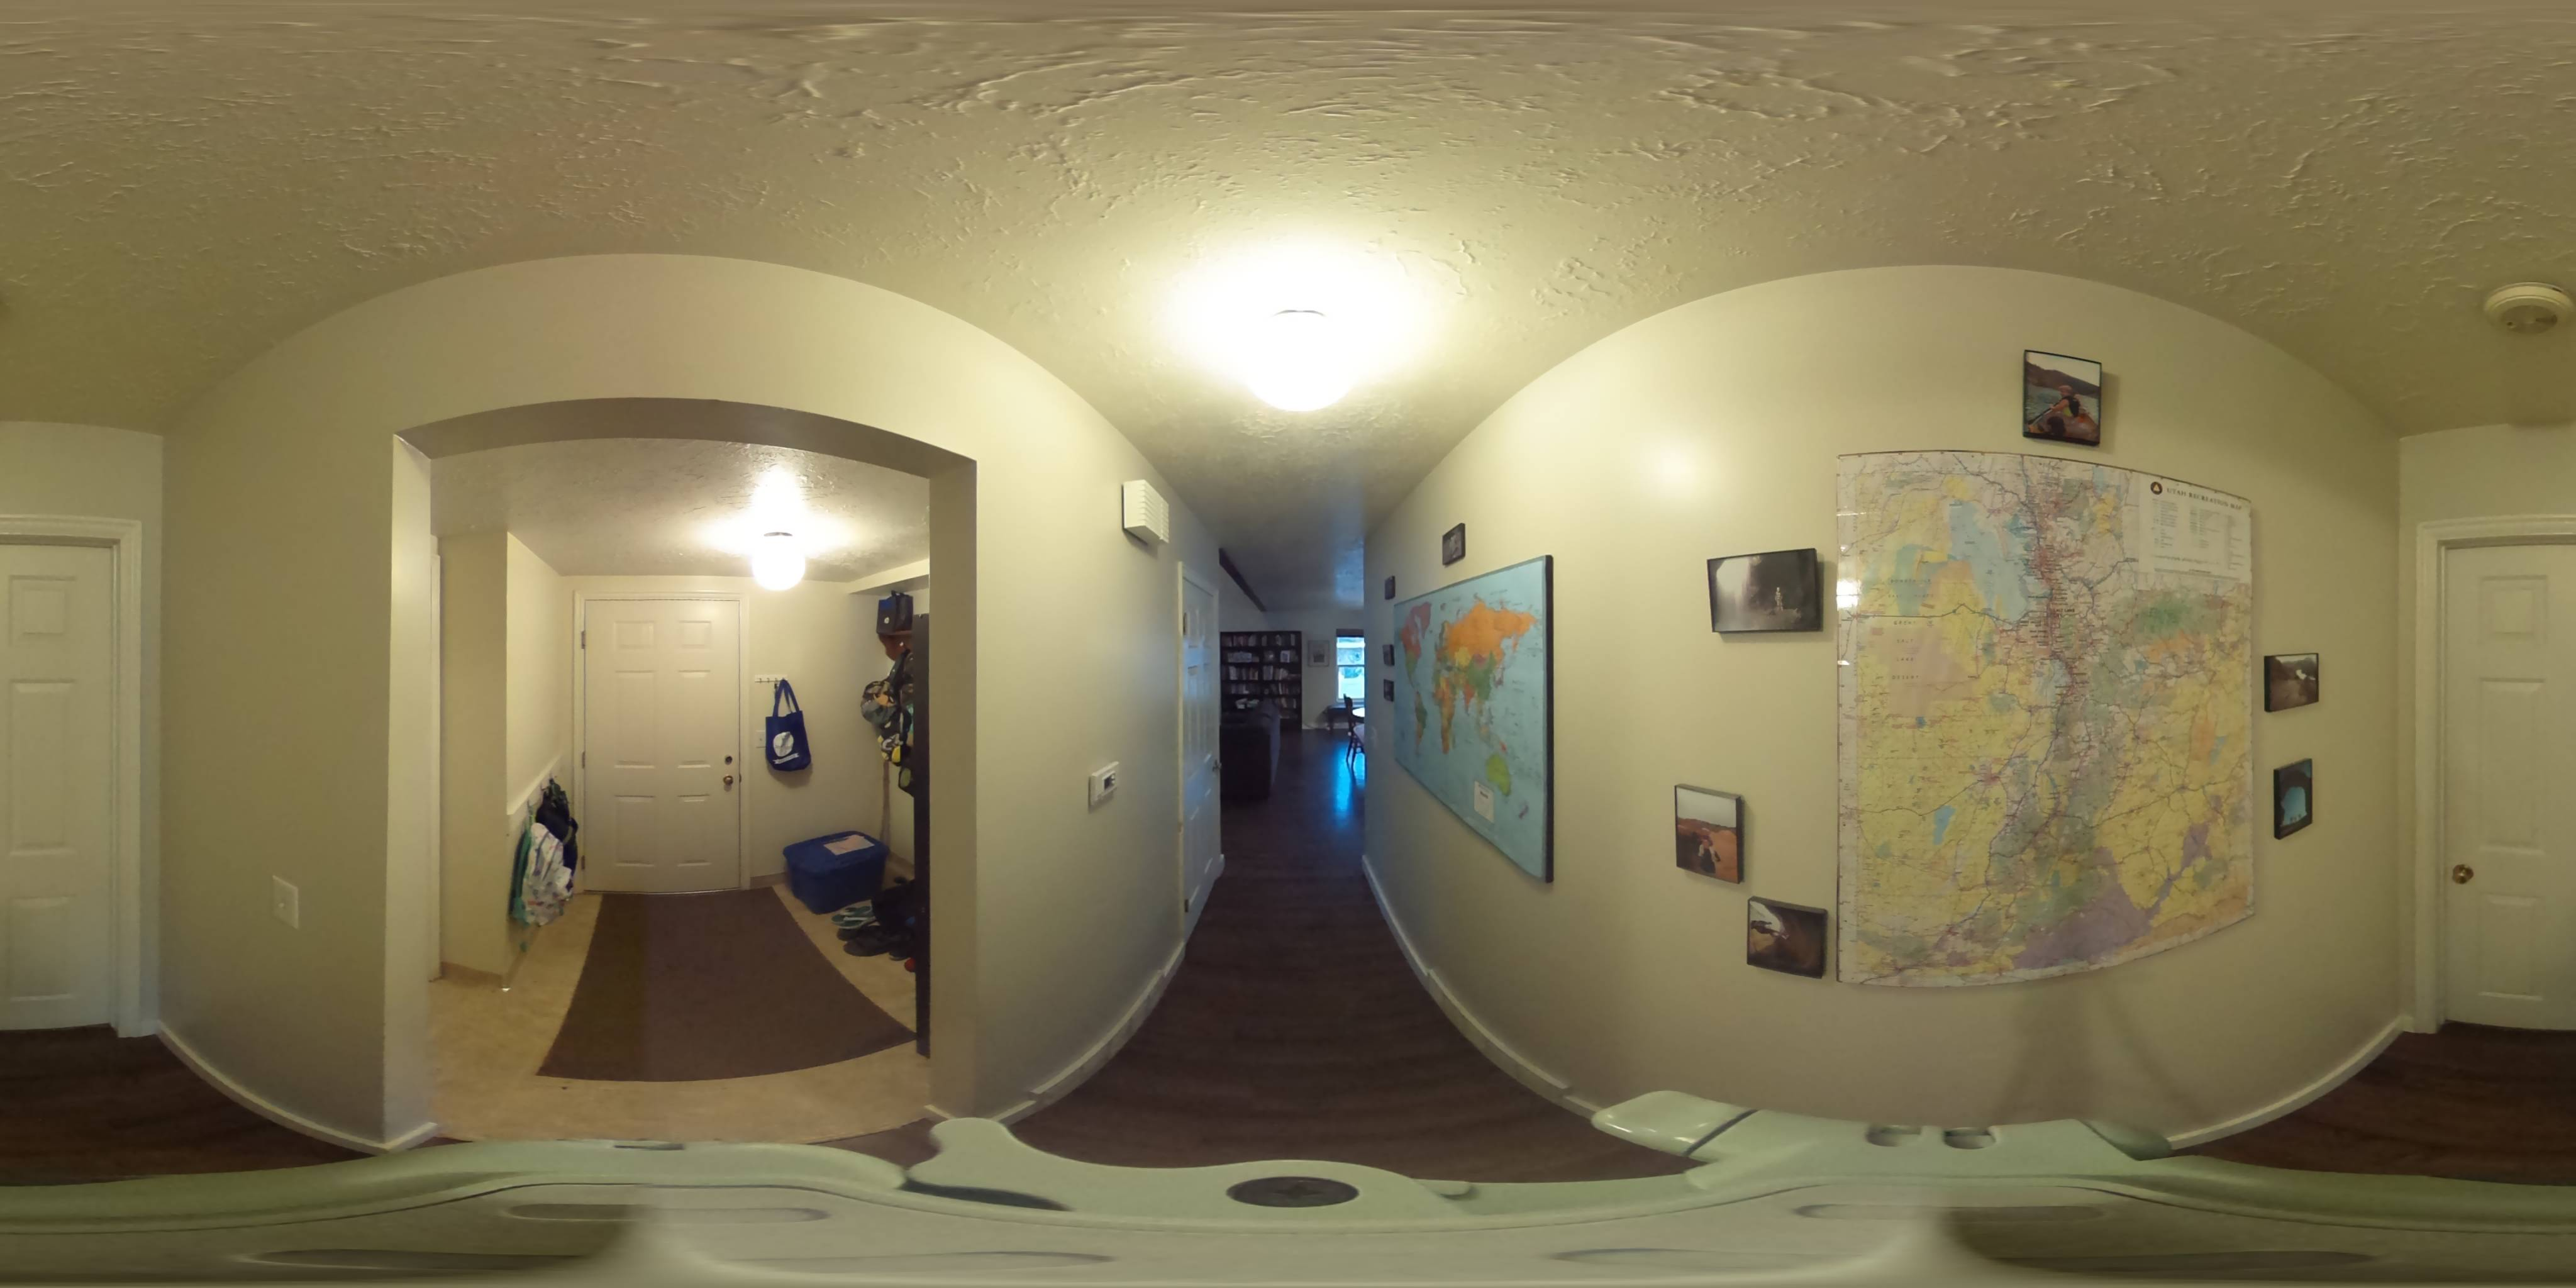
\includegraphics[width=1.0\unitlength]{Figures/equirectangular.jpg}}
       
    \end{picture}
    \caption{An example of an indoors equirectangular panorama.}
\end{figure}

\section{Environment mapping}
Environment mapping is an image-based technique to approximate the appearance of the overall light conditions of an environment. This is accomplished by means of a precomputed texture image mapped on a geometric surface as a far-away environment surrounding. This technique was originally proposed by \citep{Blinn76} using spheres. Nowadays there are other alternatives, such as cube, paraboloid, pyramid or cylinder maps. The principle of projection is similar, but the specific definition of map per surface is different.\newline
In order to generate an environment map, it is necessary that the panorama is made into a High Dynamic Range image. This is because a Low Dynamic Range image fails to capture the information necessary to simulate correct color balance, shadows, and highlights of the lighting environment; ultimately producing both inaccurate and less visually pleasing results. This has been illustrated by \citep{DebevecRSO}.\newline 
A relatively easy and effective way to make an image into an HDR version is a technique called Tone Mapping, in which versions of the same image with different exposure values are blended together to include a full range of highlights and shadows in a single image. It's important to disclaim that the Tone Mapping process does not yield an actual HDR image, but a standard 24 bit image in the $0...255$ range, with highlight and shadow valued clipped. Nevertheless, the advantage of this process is that the environment will be described in a richer way, capturing the bright areas and the shadows better than the standard exposure image.